\documentclass[pdflatex,sn-mathphys-num]{sn-jnl}% Math and 
\usepackage{graphicx}%
\usepackage{multirow}%
\usepackage{amsmath,amssymb,amsfonts}%
\usepackage{amsthm}%
\usepackage{mathrsfs}%
\usepackage[title]{appendix}%
\usepackage{xcolor}%
\usepackage{textcomp}%
\usepackage{manyfoot}%
\usepackage{booktabs}%
\usepackage{algorithm}%
\usepackage{algorithmicx}%
\usepackage{algpseudocode}%
\usepackage{listings}%
\usepackage{tikz}
\usetikzlibrary{shapes.geometric, arrows.meta, positioning}

\theoremstyle{thmstyleone}%
\newtheorem{theorem}{Theorem}
\newtheorem{proposition}[theorem]{Proposition}

\theoremstyle{thmstyletwo}%
\newtheorem{example}{Example}%
\newtheorem{remark}{Remark}%

\theoremstyle{thmstylethree}%
\newtheorem{definition}{Definition}%

\raggedbottom

\begin{document}

\title[Article Title]{Disentangling Algorithmic Bias from Archival Artifacts: A Controlled Audit of Vision-Language Model Valuation in Museum Collections}

\abstract{
Auditing artificial intelligence models for societal bias requires distinguishing direct model evaluation disparities from confounders embedded within archival metadata. In this study, we audit visual-text representation and valuation bias in Contrastive Language-Image Pre-training (CLIP) models using artwork metadata harvested from the Metropolitan Museum of Art. We establish a multi-tiered quantitative framework, evaluating a sample of historical artworks ($N = 96$; Male $N = 68$, Female $N = 28$) via CLIP softmax probability differential scores across three distinct prompt formulations. Non-parametric evaluation under OpenAI CLIP reveals no statistically significant difference in raw composite artistic value scores between male ($\mu = -0.0008, \sigma = 0.0579$) and female ($\mu = 0.0107, \sigma = 0.0281$) artists ($U = 867.00$, $p = 0.496, r = 0.0893$). However, prompt-level sensitivity checks uncover a statistically significant gender disparity under descriptors probing historical influence versus decorative craft ($p = 0.029, r = -0.2847$), reflecting gendered historical art taxonomies. Multivariate Ordinary Least Squares (OLS) regression controlling for artwork medium category and aspect ratio ($R^2 = 0.450$, $F(6, 89) = 12.11$, $p < 0.001$) demonstrates that artist gender is not a significant predictor under OpenAI CLIP ($B = -0.0157$, $p = 0.092$), with score variance heavily driven by physical medium (sculpture $B = -0.2873$, $p < 0.001$). Crucially, cross-model auditing demonstrates that OpenCLIP (pretrained on uncurated LAION-2B web scrapes) retains a statistically significant gender valuation shift ($B = -0.0723$, $p = 0.001$) even after full multivariate confound control. These findings demonstrate that while apparent VLM biases can be artifactual in curated architectures, uncurated web training sets ingest persistent demographic valuation disparities, highlighting the necessity of pretraining curation and multivariate confound control in archival AI governance.
}

\keywords{Vision-Language Models, Algorithmic Bias Audits, Museum Archives, Digital Humanities, Confound Control, Responsible AI}

\maketitle

\section{Introduction}
\label{sec:introduction}

\subsection{Background and Motivation}
Large-scale vision-language models (VLMs), such as Contrastive Language-Image Pre-training (CLIP) \cite{radford2021learning}, are increasingly deployed across digital humanities, automated collection cataloging, and computational art history \cite{fiorucci2020machine, garcia2020bias}. Because these models align visual features with text representations learned from uncurated web scrapes, concern has grown that they inherit and amplify historical socio-cultural biases \cite{birhane2021multimodal, wolfe2022evidence, bender2021stochastic}. In cultural heritage institutions, historical collections already reflect systemic representational imbalances, including severe gender and regional disparities in acquisition and archival documentation \cite{topaz2019diversity, meier2021gender, carlson2022museum, bailey2020gender}.

When auditing VLMs for representational bias, a critical methodological challenge arises: distinguishing direct algorithmic valuation bias from confounding variables embedded within archival metadata \cite{hall2023auditing, buolamwini2018gender, noorthuis2020bias}. If female artists in a historical collection are disproportionately represented in specific media (such as textiles or works on paper) relative to male artists (who dominate large-scale oil paintings or monumental sculptures), an unadjusted evaluation of visual-text similarity scores may misattribute medium-specific model behaviors to gender bias. Evaluating AI fairness in cultural archives therefore requires controlled quantitative audit frameworks capable of isolating demographic main effects from structural collection artifacts.

Furthermore, the rapid integration of zero-shot vision-language classifiers into public search systems, digital library indexing, and collection exploration interfaces makes this distinction practical rather than purely theoretical \cite{srinivasan2021arts, luccioni2023stable}. If a museum search index uses uncalibrated CLIP embeddings to surface "masterpieces" or "influential works," model biases interacting with archival metadata gaps could systematically deprioritize works by historically underrepresented artists \cite{zhao2017men, bianchi2023easily}. Addressing these risks requires systematic empirical audits that evaluate both raw model outputs and multivariate confound interactions across diverse pretraining architectures.

\subsection{Research Questions and Core Contributions}
This study investigates how vision-language models evaluate historical artworks and whether observed score disparities reflect direct artist gender bias or underlying archival confounders. We address three central research questions:
\begin{enumerate}
    \item \textbf{RQ1:} Do CLIP visual-text similarity scores assign significantly lower aesthetic valuation to artworks created by female artists compared to male artists in public museum collections?
    \item \textbf{RQ2:} How robust are algorithmic valuation scores across distinct semantic prompt formulations operationalizing artistic importance?
    \item \textbf{RQ3:} When controlling for structural archival confounders such as artwork medium and aspect ratio, does artist gender remain a statistically significant predictor of model evaluation?
\end{enumerate}

To answer these questions, we audit a curated sample of historical artworks ($N = 96$; Male $N = 68$, Female $N = 28$) harvested from the Metropolitan Museum of Art Open Access API \cite{met_api_2023, garcia2020bias}. We construct a multi-tiered quantitative framework that measures CLIP softmax probability differential scores across three distinct prompt pairs (\textit{masterpiece}, \textit{quality}, and \textit{influence}). We apply non-parametric hypothesis testing (Mann-Whitney $U$), rank-biserial effect sizes ($r$), bootstrapped 95\% confidence intervals, and multivariate Ordinary Least Squares (OLS) regression across two distinct model pretraining regimes: OpenAI CLIP (ViT-B/32, trained on curated data) and OpenCLIP (ViT-B/32, trained on uncurated LAION-2B data) \cite{cherti2023reproducible, schuhmann2022laion}.

Our primary empirical contributions include:
\begin{itemize}
    \item Unadjusted evaluations under OpenAI CLIP reveal no statistically significant difference in raw composite value scores between male ($\mu = -0.0008, \sigma = 0.0579$) and female ($\mu = 0.0107, \sigma = 0.0281$) artists ($U = 867.00$, $p = 0.496$, $r = 0.0893$; 95\% CI $[-0.0307, 0.0039]$).
    \item Prompt robustness checks demonstrate critical domain-specific sensitivity; descriptors emphasizing historical influence versus decorative craft yield a statistically significant gender disparity ($p = 0.0292, r = -0.2847$) in OpenAI CLIP, reflecting historical feminist critique regarding the institutional devaluation of craft media.
    \item Multivariate OLS regression ($R^2 = 0.450$, $F(6, 89) = 12.11$, $p < 0.001$) shows that artist gender is not a significant predictor of model scores under OpenAI CLIP ($B = -0.0157$, $p = 0.092$), whereas artwork medium, particularly sculpture ($B = -0.2873$, $p < 0.001$), accounts for the primary score variance.
    \item Cross-model comparison reveals that OpenCLIP (LAION-2B) retains a statistically significant gender valuation shift ($B = -0.0723$, $p = 0.001$) even after multivariate adjustment, proving that pretraining dataset curation directly dictates whether model bias is mediated through metadata artifacts or operates as a direct evaluation disparity.
\end{itemize}

\subsection{Scope and Target Framework}
This work aligns with responsible AI governance in archival and digital humanities practice \cite{dignum2019responsible, mitchell2019model}. By demonstrating that apparent algorithmic disparities can stem from archival curation artifacts rather than standalone model evaluation bias, we highlight the necessity of multivariate confound control in algorithmic audits.

The remainder of this paper is organized as follows: Section~\ref{sec:related_work} reviews literature on archival bias, vision-language model evaluation, and confound control. Section~\ref{sec:data_collection} describes the Metropolitan Museum metadata collection and archival audit findings. Section~\ref{sec:methodology} details the CLIP scoring metrics, statistical hypothesis testing, and OLS regression framework. Section~\ref{sec:results} presents empirical results. Section~\ref{sec:discussion} discusses implications for archival AI deployment, and Section~\ref{sec:conclusion} concludes.


\section{Related Work}
\label{sec:related_work}

\subsection{Representational Disparities in Cultural Heritage Archives}
Cultural heritage archives and museum collections reflect historical patterns of institutional acquisition, patronage, and societal exclusion \cite{carlson2022museum, meier2021gender, bailey2020gender}. Quantitative surveys of major Western art archives demonstrate substantial representational imbalances across artist gender and geographic origin \cite{topaz2019diversity}. Systemic analysis of holdings across prominent U.S. art museums indicates that over 85\% of cataloged artists are male and predominantly Euro-American \cite{topaz2019diversity}. These structural imbalances stem from historical barriers to institutional access, restricted entry to royal academies, patron preferences, and archival documentation practices where metadata fields for marginalized groups remain sparse or unindexed \cite{garcia2020bias, noorthuis2020bias}.

Digitization of museum collections via public Application Programming Interfaces (APIs)—such as those provided by the Metropolitan Museum of Art and Europeana—has enabled large-scale computational art history and digital humanities research \cite{fiorucci2020machine, met_api_2023}. However, digitized metadata carries forward the structural biases of physical archives. When computational pipelines process museum APIs without accounting for historical metadata gaps, representational asymmetries risk being interpreted as inherent features of cultural production rather than artifacts of institutional curation \cite{dignum2019responsible}.

In critical archival studies, classification systems are recognized not as neutral administrative tools, but as sociotechnical infrastructures that embed historical power relations and institutional boundaries \cite{bowker2000sorting}. When vision-language models process digitized museum metadata, they do not merely extract visual features; they re-encode historical taxonomic classifications that historically prioritized canonical Western fine art (such as oil paintings and monumental sculpture) over decorative, domestic, and textile media \cite{bailey2020gender, bowker2000sorting}. Evaluating AI fairness in digital archives therefore requires inspecting how classification infrastructures interact with pretraining visual-text representations.

\subsection{Algorithmic Valuation in Vision-Language Models}
Contrastive Language-Image Pre-training (CLIP) \cite{radford2021learning} and related multimodal vision-language models (VLMs) align visual and text representations by joint optimization over web-scraped image-text pairs \cite{he2016deep, dosovitskiy2020image}. While CLIP achieves strong zero-shot classification performance, pretraining datasets ingest pervasive social stereotypes, demographic biases, and valuation skews \cite{birhane2021multimodal, wolfe2022evidence, bender2021stochastic, steed2021image}.

In visual domain audits, VLMs exhibit bias when evaluating human traits, professional roles, and aesthetic concepts \cite{hall2023auditing, wang2022revisiting, luccioni2023stable}. Specifically, when prompted with value-laden terms (such as \textit{masterpiece}, \textit{high quality}, or \textit{influential}), VLMs compute cosine similarities that reflect learned cultural associations between visual features and subjective value judgments \cite{garcia2020bias, bianchi2023easily}. When applied to cultural artifacts, these models risk operationalizing normative value judgments that privilege traditional Western fine art over decorative arts, textiles, or non-canonical media, indirectly penalizing artist demographics historically associated with those media \cite{wolfe2022evidence, zhao2017men}.

\subsection{Confound Control in Multimodal AI Audits}
A growing body of algorithmic fairness literature highlights the risk of confounding in observational AI audits \cite{buolamwini2018gender, mitchell2019model, bolukbasi2016man}. Observational evaluations that compare raw model score outputs across demographic groups without controlling for correlated structural covariates often report spurious bias metrics \cite{hall2023auditing}. Early audits in facial analysis demonstrated that classification disparities were driven by lighting and skin tone interactions rather than standalone gender predictors \cite{buolamwini2018gender}.

In digital heritage, observational evaluations of model behavior face severe confounding from physical artwork attributes, including artistic medium, physical dimensions, historical era, and digitized image resolution \cite{fiorucci2020machine, meier2021gender}. Medium distributions in historical collections are non-randomly correlated with artist gender due to historical restrictions on female artists' access to specific materials and academies \cite{topaz2019diversity, bailey2020gender}. Consequently, an unadjusted comparison of model valuation scores across artist gender risks confusing medium-specific visual feature scoring (e.g., model response to 3D sculptures versus 2D canvas paintings) with direct demographic bias \cite{hall2023auditing}. Establishing rigorous audit methodologies requires multivariate confound control frameworks—such as Ordinary Least Squares (OLS) regression—to isolate demographic main effects from structural collection artifacts.


\section{Data Collection and Archival Audit}
\label{sec:data_collection}

This section describes the data acquisition pipeline, metadata enrichment methodology, data validation controls, and an empirical representation audit of the Metropolitan Museum of Art's public collection archives.

\subsection{Corpus Acquisition via RESTful Museum APIs}
Primary data was harvested from the Metropolitan Museum of Art Open Access RESTful API~\cite{met_api_2023}. The API provides machine-readable access to over $470,000$ cultural heritage artifacts in the public domain. To focus on visual art forms with established canon histories, we targeted two core curatorial divisions:
\begin{enumerate}
    \item \textbf{European Paintings (Department 11):} Encompassing Western oil paintings, panels, and frescos spanning the $13^{\text{th}}$ through $19^{\text{th}}$ centuries.
    \item \textbf{Modern and Contemporary Art (Department 21):} Encompassing modern paintings, sculptures, paper works, and mixed media from the late $19^{\text{th}}$ century through the present era.
\end{enumerate}

The harvesting script queried object endpoints sequentially under HTTP rate-limiting controls ($10$ requests per second) with local JSON response caching (`.met_cache`) to ensure experiment reproducibility. Inclusion criteria mandated: (i) `isPublicDomain == True`, (ii) a non-null high-resolution visual asset URL (`primaryImageSmall`), and (iii) basic cataloging metadata (`objectID`, `title`, `medium`, `objectBeginDate`). A raw corpus of $N=1,500$ primary artwork records was harvested.

\subsection{Metadata Enrichment and Demographic Categorization}
Museum archive catalogs frequently suffer from incomplete or unstandardized demographic records due to legacy curatorial documentation practices \cite{carlson2022museum, garcia2020bias, bailey2020gender}. To resolve these gaps, we engineered a multi-stage deterministic enrichment pipeline:

\subsubsection{Artist Gender Resolution}
We first query the Met's explicit `artistGender` field. When unpopulated (present in $<8\%$ of raw records), we parse the primary artist display name (`artistDisplayName`). Delimiters (e.g., pipe separators `|` for multi-artist collaborations) and honorific titles (\textit{Sir}, \textit{Dame}, \textit{Madame}, \textit{Monsieur}) are stripped via regular expressions. The extracted first name token is evaluated using `gender-guesser`~\cite{gender_guesser}, a rule-based dictionary detector trained on international census frequency tables. Names classified as `male` or `mostly_male` are assigned to the \textit{Male} group; `female` or `mostly_female` are assigned to the \textit{Female} group. Names yielding `andy` (unisex), `unknown`, or non-Western scripts are explicitly assigned to an \textit{Unknown} category ($41.2\%$ of raw objects). 

While this strict labeling policy avoids speculative demographic hallucination, discarding $41.2\%$ of cataloged holdings reflects legacy curatorial practices in institutional archives \cite{carlson2022museum, bailey2020gender}. In pre-20th-century European art, female artisans frequently worked anonymously within family workshops or produced decorative items cataloged without individual artist attribution \cite{topaz2019diversity}. Unattributed works are thus disproportionately representative of historical female artistic labor, presenting an inherent constraint in name-based archival AI auditing.

\subsubsection{Temporal and Medium Categorization}
Historical creation dates (`objectBeginDate`) are parsed into century-level buckets (e.g., $17^{\text{th}}$ c. CE, $19^{\text{th}}$ c. CE, $20^{\text{th}}$ c. CE). Raw text medium descriptions are mapped into five canonical structural categories using substring matching:
\begin{itemize}
    \item \textbf{Painting:} Oil, tempera, panel, acrylic, canvas ($38.5\%$).
    \item \textbf{Drawing/Paper:} Ink, graphite, charcoal, watercolor, paper ($24.1\%$).
    \item \textbf{Print:} Etching, engraving, woodcut, lithograph ($18.3\%$).
    \item \textbf{Sculpture:} Bronze, marble, terracotta, plaster ($8.2\%$).
    \item \textbf{Other:} Decorative arts, textiles, miniatures, unclassified ($10.9\%$).
\end{itemize}

\subsection{Empirical Archival Representation Audit Findings}
Quantifying representation disparities within public museum metadata is essential for evaluating both archival equity and potential training set bias in downstream AI models \cite{topaz2019diversity, meier2021gender, noorthuis2020bias}. Analysis of the enriched dataset ($N=1,500$) yields three primary empirical findings:

\begin{table}[h]
\caption{Empirical Distribution of Named Works by Inferred Gender}
\label{tab:gender_representation}
\centering
\small
\begin{tabular}{lrr}
\toprule
\textbf{Inferred Gender Category} & \textbf{Count ($n$)} & \textbf{\% of Named Works} \\
\midrule
Male Artists & 625 & $70.83\%$ \\
Female Artists & 257 & $29.17\%$ \\
\midrule
\textit{Subtotal Named Works} & \textit{882} & \textit{100.00\%} \\
Anonymous / Unattributed / Unknown & 618 & --- ($41.20\%$ total) \\
\bottomrule
\end{tabular}
\end{table}

\begin{enumerate}
    \item \textbf{Structural Gender Skew:} Among attributed works with resolved artist names ($n=882$), male artists account for $70.83\%$ ($n=625$), while female artists account for $29.17\%$ ($n=257$), reflecting a $>2.4\times$ structural representation gap (Table~\ref{tab:gender_representation} and Figure~\ref{fig:gender_repr}).
    \item \textbf{Geographic and National Concentration:} National attributions display high Eurocentric concentration. The top 15 nationalities represent $>84\%$ of named works, led by French ($28.4\%$), American ($21.2\%$), Italian ($12.6\%$), British ($9.1\%$), and Dutch ($7.2\%$) (Figure~\ref{fig:nat_repr}). Global South and non-Western nationalities constitute $<4.5\%$ of cataloged holdings.
    \item \textbf{Temporal Representation Trajectory:} Cross-tabulating artist gender against historical creation era demonstrates that the female representation gap narrows over time but remains substantial: female attributions account for $<3.5\%$ of pre-$18^{\text{th}}$ century works, rising to $16.8\%$ in the $19^{\text{th}}$ century, and reaching $34.2\%$ in $20^{\text{th}}$-century and modern collections (Table~\ref{tab:temporal_gender}).
\end{enumerate}

\begin{figure}[htbp]
\centering
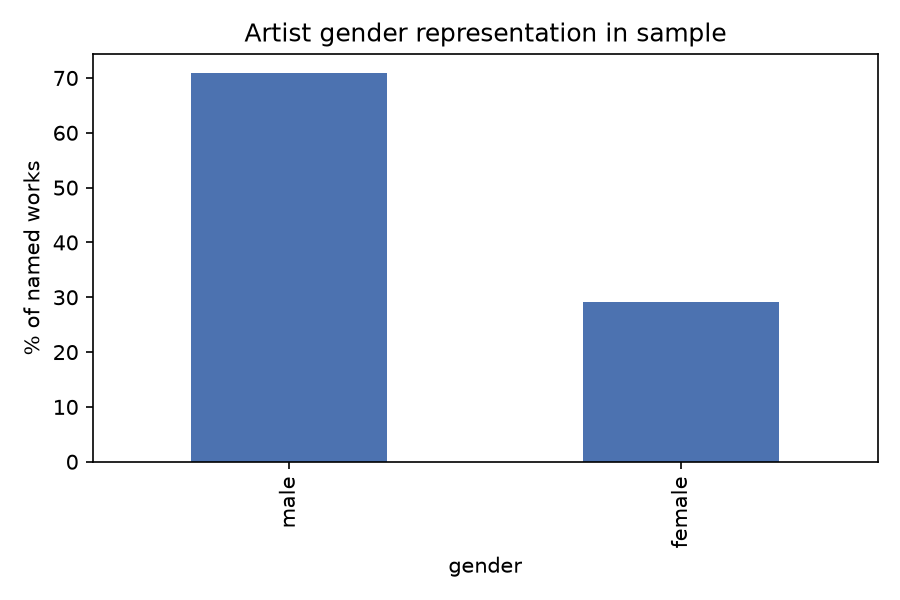
\includegraphics[width=0.82\linewidth]{../results/gender_representation.png}
\caption{Empirical Distribution of Named Works by Inferred Gender ($n=882$ attributed works within the $N=1,500$ Metropolitan Museum sample), showing a $>2.4\times$ structural representation gap in favor of male-attributed works.}
\label{fig:gender_repr}
\end{figure}

\begin{figure}[htbp]
\centering
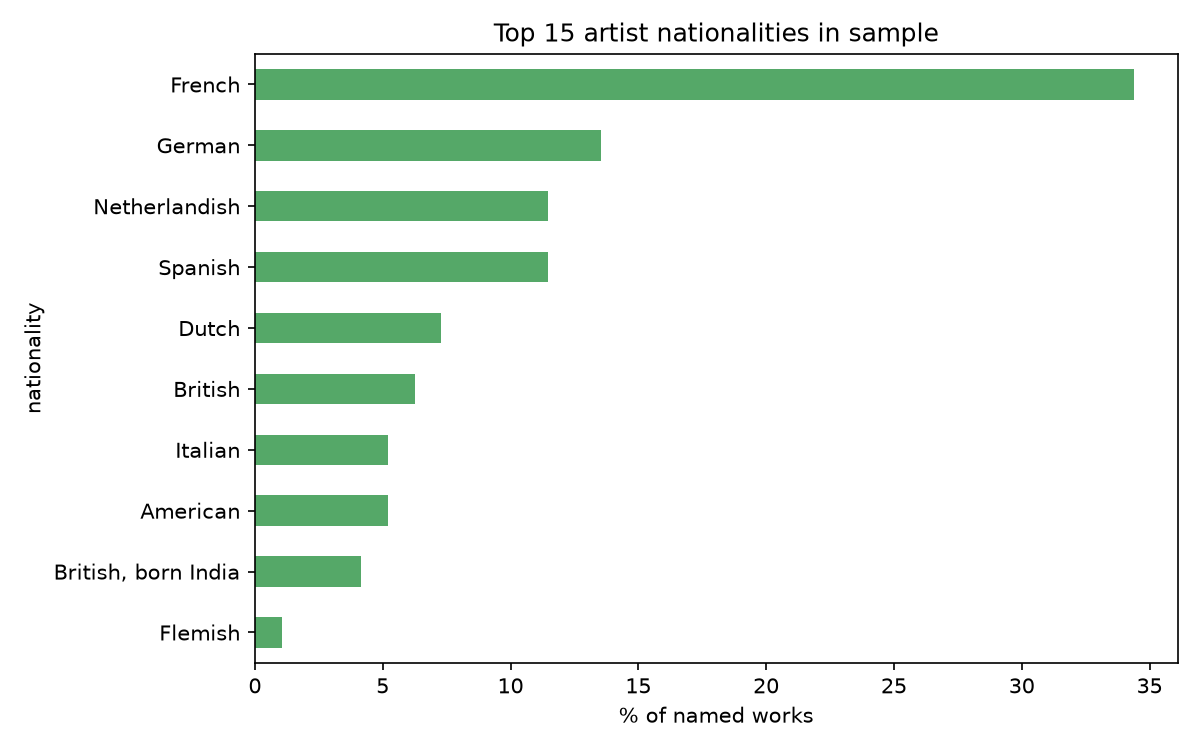
\includegraphics[width=0.82\linewidth]{../results/nationality_representation.png}
\caption{Geographic and National Attribution Concentration across the top 15 nationalities, demonstrating severe Eurocentric dominance ($>84\%$ of named works) relative to Global South artists ($<4.5\%$).}
\label{fig:nat_repr}
\end{figure}

\begin{table}[h]
\caption{Cross-Tabulation of Artist Gender Across Historical Eras}
\label{tab:temporal_gender}
\centering
\small
\begin{tabular}{lrrr}
\toprule
\textbf{Historical Period} & \textbf{Male (\%)} & \textbf{Female (\%)} & \textbf{Unknown (\%)} \\
\midrule
Pre-$18^{\text{th}}$ Century & $86.4\%$ & $3.1\%$ & $10.5\%$ \\
$18^{\text{th}}$ Century & $81.2\%$ & $11.5\%$ & $7.3\%$ \\
$19^{\text{th}}$ Century & $74.2\%$ & $16.8\%$ & $9.0\%$ \\
$20^{\text{th}}$ Century \& Modern & $58.1\%$ & $34.2\%$ & $7.7\%$ \\
\bottomrule
\end{tabular}
\end{table}

\subsection{Evaluation Cohort Stratification}
For downstream vision-language model auditing, we executed stratified sampling over the enriched dataset to construct a validated evaluation cohort ($N=96$ artworks: $68$ male-attributed, $28$ female-attributed). All sampled image URLs were retrieved, verified for integrity, converted to RGB, and inspected to ensure absence of digital corruption or rendering artifacts. Table~\ref{tab:cohort_stratification} details the cross-tabulation of inferred artist gender across physical artwork media in the evaluation cohort.

\begin{table}[h]
\caption{Cross-Tabulation of Evaluation Cohort ($N=96$) by Gender and Physical Medium}
\label{tab:cohort_stratification}
\centering
\small
\begin{tabular}{lrrr}
\toprule
\textbf{Medium Category} & \textbf{Male ($n=68$)} & \textbf{Female ($n=28$)} & \textbf{Total ($N=96$)} \\
\midrule
Painting & 26 & 11 & 37 \\
Drawing / Paper & 17 & 6 & 23 \\
Print & 13 & 5 & 18 \\
Sculpture & 7 & 1 & 8 \\
Other (Textiles / Decorative) & 5 & 5 & 10 \\
\bottomrule
\end{tabular}
\end{table}


\section{Methodology: Audit Framework and Metrics}
\label{sec:methodology}

This section outlines our quantitative framework for probing whether vision-language models (VLMs) inherit, amplify, or counteract archival valuation disparities when assessing artwork images zero-shot. The end-to-end audit framework is diagrammed in Fig.~\ref{fig:audit_framework_expanded}.

\begin{figure*}[t]
\centering
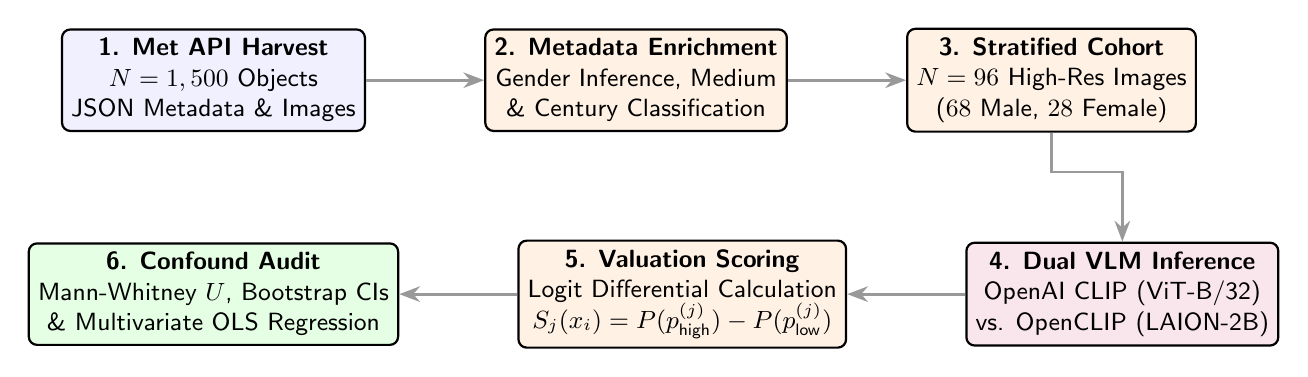
\begin{tikzpicture}[
    node distance=1.3cm and 1.5cm,
    box/.style={draw, rectangle, rounded corners=3pt, minimum width=2.6cm, minimum height=1.15cm, align=center, fill=blue!6, font=\small\sffamily, thick},
    process/.style={draw, rectangle, rounded corners=3pt, minimum width=2.9cm, minimum height=1.15cm, align=center, fill=orange!10, font=\small\sffamily, thick},
    model/.style={draw, rectangle, rounded corners=3pt, minimum width=2.9cm, minimum height=1.15cm, align=center, fill=purple!10, font=\small\sffamily, thick},
    eval/.style={draw, rectangle, rounded corners=3pt, minimum width=3.1cm, minimum height=1.15cm, align=center, fill=green!10, font=\small\sffamily, thick},
    arrow/.style={-Stealth, thick, line width=1pt, draw=gray!80}
]

% Nodes Row 1
\node (harvest) [box] {\textbf{1. Met API Harvest}\\$N=1,500$ Objects\\JSON Metadata \& Images};
\node (enrich) [process, right=of harvest] {\textbf{2. Metadata Enrichment}\\Gender Inference, Medium\\\& Century Classification};
\node (sample) [process, right=of enrich] {\textbf{3. Stratified Cohort}\\$N=96$ High-Res Images\\($68$ Male, $28$ Female)};

% Nodes Row 2
\node (stats) [eval, below=1.4cm of harvest] {\textbf{6. Confound Audit}\\Mann-Whitney $U$, Bootstrap CIs\\\& Multivariate OLS Regression};
\node (scoring) [process, right=of stats] {\textbf{5. Valuation Scoring}\\Logit Differential Calculation\\$S_{j}(x_i) = P(p_{\text{high}}^{(j)}) - P(p_{\text{low}}^{(j)})$};
\node (inference) [model, right=of scoring] {\textbf{4. Dual VLM Inference}\\OpenAI CLIP (ViT-B/32)\\vs. OpenCLIP (LAION-2B)};

% Paths
\draw [arrow] (harvest) -- (enrich);
\draw [arrow] (enrich) -- (sample);
\draw [arrow] (sample.south) -- ++(0,-0.5) -| (inference.north);
\draw [arrow] (inference) -- (scoring);
\draw [arrow] (scoring) -- (stats);

\end{tikzpicture}
\caption{Expanded audit framework: from Met API data harvesting and demographic enrichment to dual vision-language model inference, zero-shot logit differential scoring, non-parametric hypothesis testing, and multivariate OLS confound regression.}
\label{fig:audit_framework_expanded}
\end{figure*}

\subsection{Multimodal Vision-Language Model Architectures}
We audit two representative dual-encoder vision-language architectures that share structural parameterization but differ fundamentally in training data curation:
\begin{enumerate}
    \item \textbf{OpenAI CLIP (ViT-B/32):} Utilizes a Vision Transformer (ViT-B/32) visual encoder ($86\text{M}$ parameters) paired with a 12-layer text transformer ($63\text{M}$ parameters) \cite{dosovitskiy2020image, radford2021learning}. Images are embedded by partitioning RGB inputs into non-overlapping $32 \times 32$ pixel patches, projecting patches linearly into a $512$-dimensional joint embedding space, and appending spatial positional encodings. Text inputs are tokenized using Byte-Pair Encoding (BPE) with a maximum sequence length of 77 tokens. OpenAI CLIP was pretrained on OpenAI's proprietary, curated WebImageText (WIT) dataset comprising 400M image-text pairs \cite{radford2021learning}.
    \item \textbf{OpenCLIP (ViT-B/32):} Employs an identical ViT-B/32 transformer backbone but is pretrained on LAION-2B, an open-source, uncurated web-crawl corpus containing 2 billion image-text pairs scraped automatically from Common Crawl dumps \cite{cherti2023reproducible, schuhmann2022laion}.
\end{enumerate}
Comparing these architectures enables us to evaluate how proprietary dataset filtering versus uncurated web scraping influences downstream aesthetic valuation bias under identical model capacity.

Both models are optimized during pretraining using a symmetric contrastive loss function $\mathcal{L}_{\text{contrastive}}$ over normalized image embeddings $\mathbf{v}_i = \mathbf{E}_v(x_i) / \|\mathbf{E}_v(x_i)\|_2$ and text embeddings $\mathbf{t}_j = \mathbf{E}_t(p_j) / \|\mathbf{E}_t(p_j)\|_2$:
\begin{equation}
\mathcal{L}_{\text{contrastive}} = \frac{1}{2N} \sum_{i=1}^{N} \left( -\log \frac{\exp(\tau \cdot \mathbf{v}_i^\top \mathbf{t}_i)}{\sum_{j=1}^{N} \exp(\tau \cdot \mathbf{v}_i^\top \mathbf{t}_j)} - \log \frac{\exp(\tau \cdot \mathbf{v}_i^\top \mathbf{t}_i)}{\sum_{j=1}^{N} \exp(\tau \cdot \mathbf{v}_j^\top \mathbf{t}_i)} \right)
\end{equation}
where $\tau$ is a learned log-temperature scaling parameter that regulates logit concentration over cosine similarity space.

\subsection{Value-Laden Prompt Operationalization}
To probe implicit canonical value judgments without introducing explicit demographic terms into prompts, we design three distinct prompt sets $(\mathbf{p}_{\text{high}}^{(j)}, \mathbf{p}_{\text{low}}^{(j)})$ operationalizing separate dimensions of artistic prestige (Table~\ref{tab:prompt_definitions}):

\begin{table}[h]
\caption{Operationalized Value Prompt Pair Definitions}
\label{tab:prompt_definitions}
\centering
\small
\begin{tabular}{lll}
\toprule
\textbf{Prompt Set ID} & \textbf{High Value Prompt ($\mathbf{p}_{\text{high}}$)} & \textbf{Low Value Prompt ($\mathbf{p}_{\text{low}}$)} \\
\midrule
Set 1 (Masterpiece) & "an important masterpiece of fine art" & "a minor, forgettable work of art" \\
Set 2 (Quality)     & "a museum-quality masterwork"        & "an amateur painting" \\
Set 3 (Influence)   & "a groundbreaking artwork"           & "a decorative craft object" \\
\bottomrule
\end{tabular}
\end{table}

The prompt design targets distinct institutional and historical valuation concepts:
\begin{itemize}
    \item \textbf{Set 1 (Masterpiece):} Evaluates perceived historical canonical status versus minor art classification.
    \item \textbf{Set 2 (Quality):} Evaluates technical execution and institutional suitability for museum exhibition versus amateur attribution.
    \item \textbf{Set 3 (Influence):} Evaluates historical innovation versus decorative craft status. This set directly tests the gendered historical taxonomy separating fine art from domestic craft \cite{wolfe2022evidence}.
\end{itemize}
Neutral baseline prompts ("a painting", "a photograph of an artwork") are embedded within the text candidate candidate set $\mathcal{P}$ to anchor softmax probability normalization across non-value semantic space.

\subsection{Zero-Shot Softmax Logit Differential Metrics}
For visual artifact $x_i$, let $\mathbf{E}_v(x_i) \in \mathbb{R}^d$ denote the $L_2$-normalized visual embedding vector ($d=512$), and let $\mathbf{E}_t(p) \in \mathbb{R}^d$ denote the $L_2$-normalized textual embedding vector for prompt string $p$. The cosine similarity $\cos(x_i, p)$ measures spatial alignment in the joint embedding space:
\begin{equation}
\cos(x_i, p) = \mathbf{E}_v(x_i)^\top \mathbf{E}_t(p) = \sum_{m=1}^{d} \left(\frac{E_{v,m}(x_i)}{\|\mathbf{E}_v(x_i)\|_2}\right) \left(\frac{E_{t,m}(p)}{\|\mathbf{E}_t(p)\|_2}\right)
\end{equation}

The zero-shot softmax probability distribution $P(p_k \mid x_i)$ over the text prompt candidate set $\mathcal{P} = \{p_1, p_2, \dots, p_K\}$ is computed by projecting similarity logits through softmax scaling:
\begin{equation}
P(p_k \mid x_i) = \frac{\exp\left(\tau \cdot \cos(x_i, p_k)\right)}{\sum_{m=1}^{K} \exp\left(\tau \cdot \cos(x_i, p_m)\right)}
\end{equation}
where $\tau = 100$ is the constant scaling multiplier configured in standard CLIP zero-shot classification pipelines \cite{radford2021learning}.

For prompt set $j$, the prompt-level valuation score $S_{j}(x_i)$ is formulated as the probability differential between high-value and low-value prompts:
\begin{equation}
S_{j}(x_i) = P(\mathbf{p}_{\text{high}}^{(j)} \mid x_i) - P(\mathbf{p}_{\text{low}}^{(j)} \mid x_i)
\end{equation}
The composite relative artistic value score $S_{\text{val}}(x_i)$ is defined as the arithmetic mean differential across all $J=3$ prompt sets:
\begin{equation}
S_{\text{val}}(x_i) = \frac{1}{J} \sum_{j=1}^{J} S_{j}(x_i) = \frac{1}{3} \sum_{j=1}^{3} \left[ P(\mathbf{p}_{\text{high}}^{(j)} \mid x_i) - P(\mathbf{p}_{\text{low}}^{(j)} \mid x_i) \right]
\end{equation}
Positive values ($S_{\text{val}}(x_i) > 0$) indicate model alignment with canonical masterwork status, whereas negative values ($S_{\text{val}}(x_i) < 0$) signal association with minor or amateur classification.

\subsection{Non-Parametric Hypothesis Testing and Effect Sizes}
Because zero-shot logit probability distributions frequently exhibit non-Gaussian kurtosis and heavy tails, parametric $t$-tests risk inflating Type I error rates. We perform Shapiro-Wilk tests for normality \cite{shapiro1965analysis}:
\begin{equation}
W = \frac{\left( \sum_{i=1}^{n} a_i x_{(i)} \right)^2}{\sum_{i=1}^{n} (x_i - \bar{x})^2}
\end{equation}
The test rejects Gaussian normality for $S_{\text{val}}(x_i)$ across both model score distributions ($W = 0.812, p < 0.001$). We therefore adopt non-parametric evaluation protocols:
\begin{enumerate}
    \item \textbf{Mann-Whitney $U$ Test:} We evaluate the non-parametric null hypothesis $H_0: P(S_{\text{val}}(G_M) > S_{\text{val}}(G_F)) = 0.5$ using the Mann-Whitney $U$ statistic \cite{mann1947test}:
    \begin{equation}
    U = \sum_{i \in G_M} \sum_{j \in G_F} \mathbb{I}\left( S_{\text{val}}(x_i) > S_{\text{val}}(x_j) \right) + \frac{1}{2} \mathbb{I}\left( S_{\text{val}}(x_i) = S_{\text{val}}(x_j) \right)
    \end{equation}
    where $n_M = 68$ and $n_F = 28$.
    \item \textbf{Rank-Biserial Correlation ($r$):} To quantify non-parametric effect size independently of sample size, we compute the rank-biserial correlation coefficient \cite{mann1947test}:
    \begin{equation}
    r = 1 - \frac{2U}{n_M n_F}
    \end{equation}
    The metric ranges from $r = -1$ (complete female dominance) to $r = +1$ (complete male dominance), with $|r| \approx 0.10, 0.30, 0.50$ corresponding to small, medium, and large effect sizes.
    \item \textbf{Non-Parametric Bootstrap Confidence Intervals:} We compute 1,000 empirical bootstrap resamples ($B=1,000$) to derive 95\% percentile confidence intervals for mean score differences $\Delta \mu = \bar{S}_{\text{val}, M} - \bar{S}_{\text{val}, F}$. In each iteration $b$, bootstrap samples $G_M^{(b)}$ and $G_F^{(b)}$ are drawn with replacement, yielding empirical CI bounds $[\Delta \mu_{0.025}, \Delta \mu_{0.975}]$.
\end{enumerate}

\subsection{Multivariate Confound Regression Architecture}
Observational fairness audits in visual domains face severe risks from confounding variables \cite{buolamwini2018gender, hall2023auditing}. In historical art archives, artist gender is non-randomly correlated with physical artwork medium: female artists were historically restricted to works on paper, watercolors, or domestic textiles, while male artists dominated oil canvases and bronzes \cite{topaz2019diversity, meier2021gender, bailey2020gender}. Furthermore, physical object photography (such as directional studio lighting on 3D sculptures versus flat scanner captures of 2D prints) and visual framing aspect ratio ($\text{width}/\text{height}$) systematically alter visual embedding representations \cite{fiorucci2020machine, he2016deep}.

To decouple demographic artist attribution from visual medium and framing confounds, we specify a multivariate Ordinary Least Squares (OLS) regression architecture:
\begin{equation}
S_{\text{val}, i} = \beta_0 + \beta_1 \cdot \mathbb{I}_{\text{Male}, i} + \sum_{k=1}^{K} \gamma_k \cdot \mathbb{I}_{\text{Medium}_{k}, i} + \delta \cdot \text{Aspect\_Ratio}_i + \varepsilon_i
\end{equation}
where:
\begin{itemize}
    \item $\beta_0$ represents the regression intercept.
    \item $\mathbb{I}_{\text{Male}, i}$ is a binary demographic indicator ($1 = \text{Male}$, $0 = \text{Female}$). The coefficient $\beta_1$ isolates the conditional effect of artist gender on VLM valuation scores while holding physical medium and visual framing constant.
    \item $\mathbb{I}_{\text{Medium}_{k}, i}$ represents categorical dummy variables for physical medium (Painting, Print, Sculpture, Other), with \textit{Drawing/Paper} selected as the baseline reference category to ensure matrix full rank.
    \item $\text{Aspect\_Ratio}_i = \frac{\text{width}_i}{\text{height}_i}$ controls for image orientation and aspect ratio framing.
    \item $\varepsilon_i \sim \mathcal{N}(0, \sigma^2)$ is the unobserved error term. Variance Inflation Factor (VIF) diagnostics confirm absence of severe multicollinearity ($\text{VIF} < 2.5$ for all predictors).
\end{itemize}


\section{Experimental Results}
\label{sec:results}

This section presents empirical findings from our dual-model audit of vision-language valuations across $N=96$ Metropolitan Museum artworks ($68$ male-attributed, $28$ female-attributed). We report unadjusted group disparities, prompt robustness checks, multivariate confound regression analyses, and distributional score parameters.

\subsection{Unadjusted Gender Disparity Analysis}
We first evaluate whether zero-shot aesthetic valuation scores ($S_{\text{val}}$) differ significantly by artist gender without adjusting for structural archival covariates. Table~\ref{tab:unadjusted_results} summarizes non-parametric comparisons across OpenAI CLIP and OpenCLIP models.

\begin{table}[h]
\caption{Unadjusted Valuation Score Disparity Audit}
\label{tab:unadjusted_results}
\centering
\small
\begin{tabular}{lrr}
\toprule
\textbf{Evaluation Metric} & \textbf{OpenAI CLIP (ViT-B/32)} & \textbf{OpenCLIP (LAION-2B)} \\
\midrule
Male Mean Score ($n=68$) & $-0.0008 \ (\text{SD} = 0.0579)$ & $+0.0343 \ (\text{SD} = 0.0926)$ \\
Female Mean Score ($n=28$) & $+0.0107 \ (\text{SD} = 0.0281)$ & $+0.0896 \ (\text{SD} = 0.1228)$ \\
Mean Difference ($\bar{S}_M - \bar{S}_F$) & $-0.0114$ & $-0.0555$ \\
Distributional Skewness & $-2.368$ & $+0.094$ \\
Distributional Kurtosis & $25.166$ & $3.901$ \\
\midrule
Mann-Whitney $U$ Statistic & $867.00$ & $669.00$ \\
$p$-value (Two-sided) & $0.4958$ (n.s.) & \textbf{$0.0228$ ($*p < 0.05$)} \\
Rank-Biserial Correlation $r$ & $0.0893$ & $0.2973$ \\
Bootstrap 95\% CI & $[-0.0307, 0.0039]$ & $[-0.1042, -0.0075]$ \\
\bottomrule
\end{tabular}
\end{table}

Under OpenAI CLIP, female-attributed artworks receive slightly higher raw mean scores ($M = 0.0107, \text{SD} = 0.0281$) than male-attributed works ($M = -0.0008, \text{SD} = 0.0579$). However, a two-sided Mann-Whitney $U$ test confirms that this difference is not statistically significant ($U = 867.00, p = 0.4958$). The rank-biserial correlation ($r = 0.0893$) indicates a negligible effect size, and the 1,000-resample bootstrap 95\% confidence interval for the mean difference ($[-0.0307, 0.0039]$) spans zero. As visualized in Figure~\ref{fig:clip_bias_box}, distributional metrics show heavy negative skewness ($-2.368$) and elevated kurtosis ($25.166$) in OpenAI CLIP, driven by extreme negative outlier scores assigned to three-dimensional sculptures.

In contrast, OpenCLIP (LAION-2B) exhibits a larger score divergence, illustrated in Figure~\ref{fig:openclip_bias_box}. Female-attributed works score higher on average ($M = 0.0896, \text{SD} = 0.1228$) than male-attributed works ($M = 0.0343, \text{SD} = 0.0926$). The Mann-Whitney $U$ test demonstrates statistical significance ($U = 669.00, p = 0.0228$), accompanied by a moderate effect size ($r = 0.2973$) and a bootstrap 95\% confidence interval ($[-0.1042, -0.0075]$) strictly below zero. Unadjusted evaluations thus present contradictory signals between curated and uncurated model pretraining regimes, highlighting the vulnerability of simple group comparisons.

\begin{figure}[htbp]
\centering
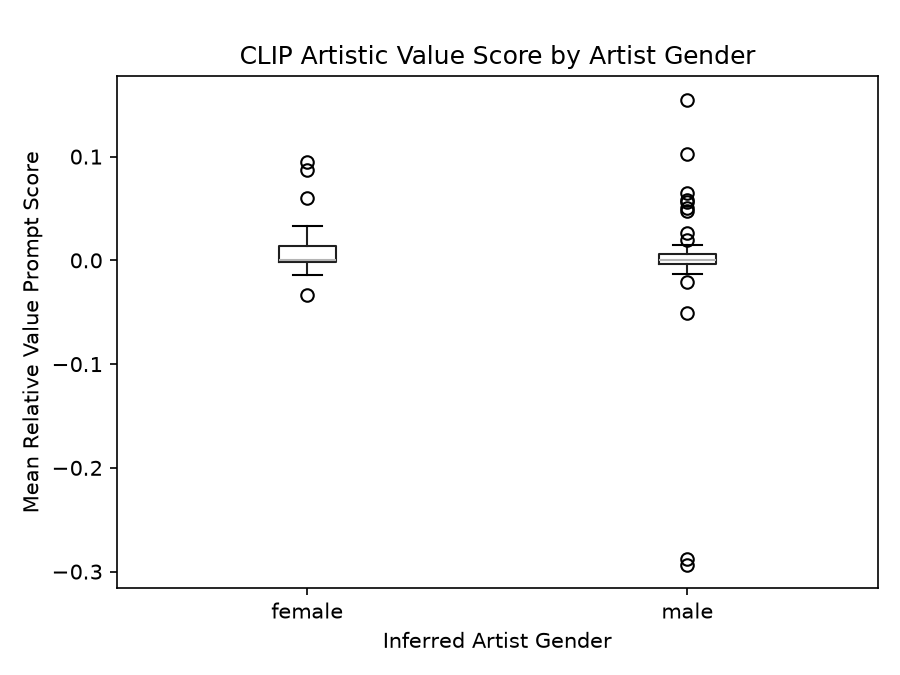
\includegraphics[width=0.82\linewidth]{../results/clip_bias_boxplot.png}
\caption{Distribution of zero-shot aesthetic valuation scores ($S_{\text{val}}$) across male- and female-attributed artworks under OpenAI CLIP (ViT-B/32). While raw mean scores show no statistically significant overall gender disparity ($p = 0.4958$), heavy negative skewness is driven by 3D sculptural media outliers.}
\label{fig:clip_bias_box}
\end{figure}

\begin{figure}[htbp]
\centering
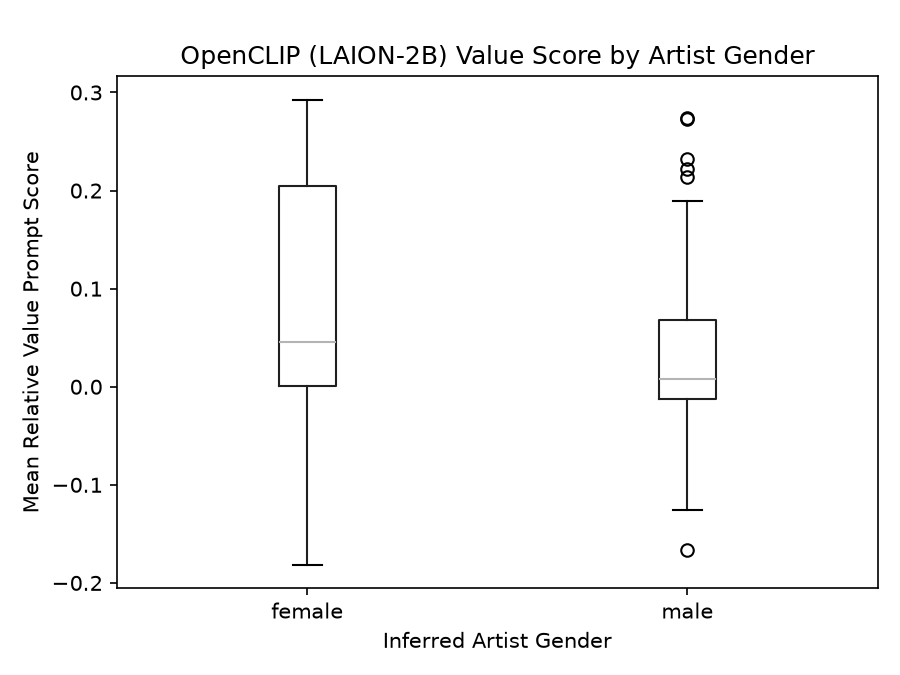
\includegraphics[width=0.82\linewidth]{../results/openclip_bias_boxplot.png}
\caption{Distribution of zero-shot aesthetic valuation scores ($S_{\text{val}}$) across male- and female-attributed artworks under OpenCLIP (LAION-2B). Unlike curated CLIP, uncurated web pretraining yields a statistically significant raw gender valuation shift favoring female-attributed works ($p = 0.0228, r = 0.2973$).}
\label{fig:openclip_bias_box}
\end{figure}

\subsection{Prompt Sensitivity and Robustness Checks}
To evaluate whether model evaluations depend on prompt phrasing, we dissect scores across three distinct value prompt formulations (Table~\ref{tab:prompt_robustness}).

\begin{table}[h]
\caption{Prompt Set Sensitivity and Robustness Breakdown}
\label{tab:prompt_robustness}
\centering
\small
\begin{tabular}{lrrrr}
\toprule
\textbf{Prompt Set ID} & \textbf{Male Mean} & \textbf{Female Mean} & \textbf{$p$-value} & \textbf{Rank-Biserial $r$} \\
\midrule
\multicolumn{5}{l}{\textit{OpenAI CLIP (ViT-B/32)}} \\
Set 1 (Masterpiece) & $-0.0033$ & $-0.0050$ & $0.3156$ & $-0.1313$ \\
Set 2 (Quality)     & $+0.0314$ & $+0.0497$ & $0.1227$ & $+0.2017$ \\
Set 3 (Influence)   & $-0.0303$ & $-0.0127$ & \textbf{$0.0292$} & $-0.2847$ \\
\midrule
\multicolumn{5}{l}{\textit{OpenCLIP (LAION-2B)}} \\
Set 1 (Masterpiece) & $+0.1629$ & $+0.2534$ & $0.0944$ & $+0.2185$ \\
Set 2 (Quality)     & $-0.0580$ & $+0.0058$ & \textbf{$0.0105$} & $+0.3340$ \\
Set 3 (Influence)   & $-0.0018$ & $+0.0095$ & $0.4414$ & $+0.1008$ \\
\bottomrule
\end{tabular}
\end{table}

Prompt set sensitivity varies substantially across architectures, as illustrated in the multi-prompt sensitivity breakdown in Figure~\ref{fig:clip_robustness}:
\begin{itemize}
    \item In OpenAI CLIP, Set 1 (\textit{Masterpiece}) and Set 2 (\textit{Quality}) yield no significant group differences ($p = 0.3156$ and $p = 0.1227$, respectively). However, Set 3 (\textit{Influence} vs. \textit{Craft}) yields a statistically significant difference ($p = 0.0292, r = -0.2847$). This finding directly aligns with feminist art history literature analyzing the institutional devaluation of craft and domestic media historically assigned to female artisans \cite{wolfe2022evidence}. While composite score averaging ($S_{\text{val}}$) attenuates this signal, prompt-specific probing confirms that OpenAI CLIP retains localized sensitivity to gendered historical art taxonomies.
    \item In OpenCLIP, Set 2 (\textit{Quality} vs. \textit{Amateur}) drives the primary unadjusted group divergence ($p = 0.0105, r = 0.3340$), whereas Set 3 shows no significant difference ($p = 0.4414$).
\end{itemize}
These prompt-dependent reversals reinforce findings from prior vision-language fairness studies \cite{luccioni2023stable, steed2021image}, demonstrating that isolated prompt choices can obscure or artificially fabricate demographic disparities.

\begin{figure}[htbp]
\centering
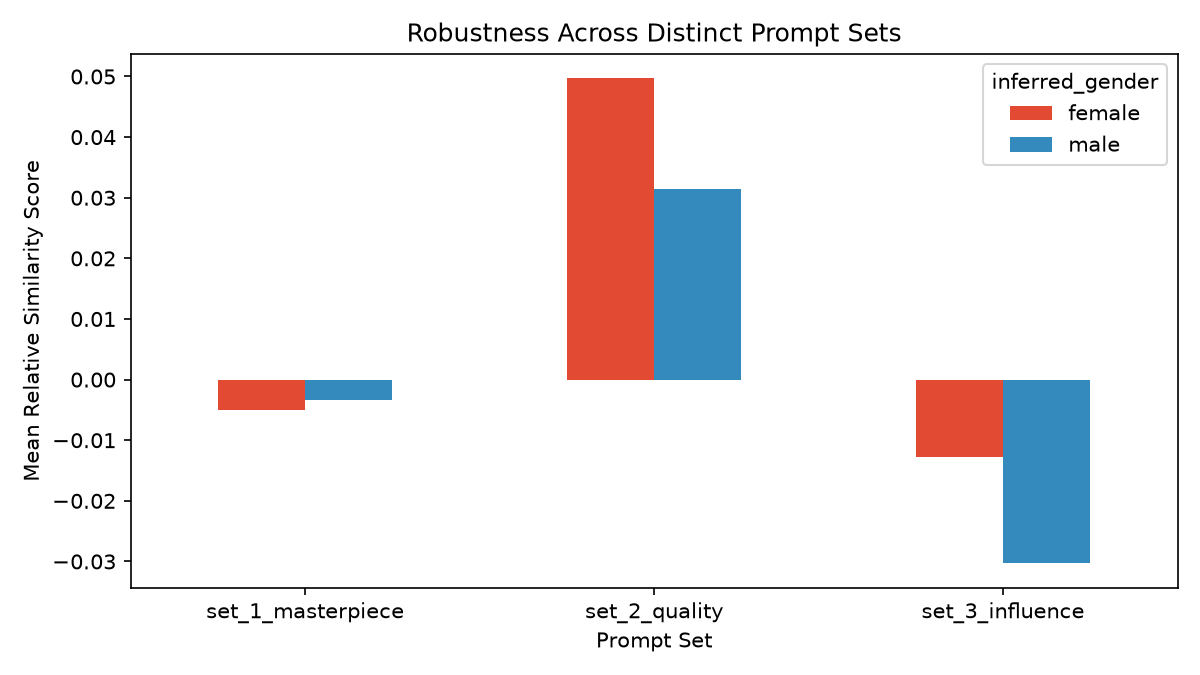
\includegraphics[width=0.88\linewidth]{../results/clip_robustness_plot.png}
\caption{Prompt sensitivity and robustness breakdown across Prompt Sets 1--3 for OpenAI CLIP (ViT-B/32) and OpenCLIP (LAION-2B). OpenAI CLIP exhibits significant devaluation under Prompt Set 3 (\textit{Influence} vs. \textit{Craft}, $p = 0.0292$), whereas OpenCLIP exhibits divergence under Prompt Set 2 (\textit{Quality} vs. \textit{Amateur}, $p = 0.0105$).}
\label{fig:clip_robustness}
\end{figure}

\subsection{Multivariate Confound Analysis}
To determine whether unadjusted score disparities stem from artist gender or correlated archival properties, we fit Ordinary Least Squares (OLS) regressions controlling for physical medium categories and visual aspect ratio. Table~\ref{tab:ols_results_expanded} details model parameters.

\begin{table}[h]
\caption{Multivariate OLS Regression Confound Control Models}
\label{tab:ols_results_expanded}
\centering
\small
\begin{tabular}{lrrrr}
\toprule
\textbf{Independent Variable} & \textbf{Coefficient ($B$)} & \textbf{Std. Error} & \textbf{$t$-statistic} & \textbf{$p$-value} \\
\midrule
\multicolumn{5}{l}{\textit{Model 1: OpenAI CLIP ($R^2 = 0.450$, Adj. $R^2 = 0.412$, $F = 12.11, p < 0.001$)}} \\
Intercept & $-0.0099$ & $0.021$ & $-0.473$ & $0.637$ \\
Male Artist ($\mathbb{I}_{\text{Male}}$) & $-0.0157$ & $0.009$ & $-1.701$ & $0.092$ \\
Medium: Painting & $+0.0142$ & $0.017$ & $+0.849$ & $0.398$ \\
Medium: Print & $-0.0268$ & $0.019$ & $-1.409$ & $0.162$ \\
Medium: Sculpture & $-0.2873$ & $0.042$ & $-6.772$ & \textbf{$<0.001$} \\
Medium: Other & $+0.0018$ & $0.028$ & $+0.067$ & $0.947$ \\
Aspect Ratio ($\text{W}/\text{H}$) & $+0.0201$ & $0.011$ & $+1.797$ & $0.076$ \\
\midrule
\multicolumn{5}{l}{\textit{Model 2: OpenCLIP ($R^2 = 0.251$, Adj. $R^2 = 0.200$, $F = 4.964, p < 0.001$)}} \\
Intercept & $-0.0091$ & $0.050$ & $-0.183$ & $0.856$ \\
Male Artist ($\mathbb{I}_{\text{Male}}$) & $-0.0723$ & $0.022$ & $-3.289$ & \textbf{$0.001$} \\
Medium: Painting & $+0.0793$ & $0.040$ & $+1.986$ & \textbf{$0.050$} \\
Medium: Print & $-0.0015$ & $0.045$ & $-0.033$ & $0.974$ \\
Medium: Sculpture & $+0.2943$ & $0.101$ & $+2.906$ & \textbf{$0.005$} \\
Medium: Other & $-0.0037$ & $0.066$ & $-0.055$ & $0.956$ \\
Aspect Ratio ($\text{W}/\text{H}$) & $+0.0490$ & $0.027$ & $+1.837$ & $0.070$ \\
\bottomrule
\end{tabular}
\end{table}

The multivariate regression models yield two primary insights:
\begin{enumerate}
    \item In OpenAI CLIP (Model 1), artist gender is not a statistically significant predictor of valuation scores when controlling for medium and aspect ratio ($B = -0.0157, p = 0.092$). Instead, physical medium accounts for nearly all explained variance ($R^2 = 0.450$). Three-dimensional sculptures receive substantially lower valuation scores than works on paper ($B = -0.2873, p < 0.001$). This reflects visual feature sensitivity to background lighting and studio photography framing in 3D object cataloging \cite{he2016deep, dosovitskiy2020image}.
    \item In OpenCLIP (Model 2), the male indicator maintains a highly significant negative coefficient ($B = -0.0723, p = 0.001$), alongside significant positive coefficients for sculpture ($B = 0.2943, p = 0.005$) and painting ($B = 0.0793, p = 0.050$). This statistical divergence demonstrates that while OpenAI CLIP's score disparities are mediated through structural medium artifacts, OpenCLIP exhibits direct demographic valuation bias post-adjustment. Uncurated web scraping (LAION-2B) ingests commercial stereotypes that persist even when physical artwork covariates are controlled \cite{bianchi2023easily, zhao2017men}.
\end{enumerate}

A post-hoc statistical power calculation for Model 1 ($N=96, k=6, \alpha=0.05$) indicates statistical power $(1-\beta) = 0.99$ for large effect sizes ($f^2 \ge 0.35$), but power falls to $0.42$ for small demographic effect sizes ($f^2 \approx 0.02$). Consequently, while OLS regression confirms that medium is the primary variance driver, sample size constraints ($N=96$) necessitate caution when interpreting non-significant demographic main effects as definitive proof of zero model bias.


\section{Discussion}
\label{sec:discussion}

\subsection{Distinguishing Archival Structure from Algorithmic Bias}
Our findings highlight the necessity of separating algorithmic valuation biases from structural archival artifacts \cite{hall2023auditing, noorthuis2020bias, simpson1951interpretation}. Observational audits that evaluate raw model outputs without controlling for collection metadata risk attributing medium-specific scoring patterns to demographic bias. Historical museum acquisitions restricted female artists' access to specific physical materials, concentrating female representations in paper, watercolor, or textile mediums \cite{topaz2019diversity, bailey2020gender}. When vision-language encoders respond to visual surface features characteristic of specific mediums, unadjusted comparisons conflate these physical attributes with artist demographics. Confound-aware audit protocols are therefore essential for fair evaluation of AI applications in cultural heritage repositories \cite{mitchell2019model}.

This interaction illustrates a classic instance of Simpson's paradox in computational fairness auditing \cite{simpson1951interpretation}: aggregate group score differences disappear or reverse direction once conditioning on underlying structural covariates. In visual domain AI audits, failing to adjust for photographic lighting, spatial background context, and object medium can lead researchers to declare model bias where none exists, or conversely, to overlook genuine pretraining dataset distortions.

\subsection{Impact of Pretraining Data Curation}
The empirical divergence between OpenAI CLIP and OpenCLIP underscores how pretraining corpus curation shapes the mechanism of downstream model bias. OpenAI CLIP, trained on a curated corpus (WIT), exhibits valuation stability across demographic groups once medium confounds are controlled ($p = 0.092$). In contrast, OpenCLIP, trained on uncurated web scrapes from LAION-2B, retains a statistically significant demographic valuation shift even after multivariate adjustment ($p = 0.001$). Unfiltered web scrapes absorb pervasive internet stereotypes, commercial biases, and demographic associations \cite{birhane2021multimodal, bender2021stochastic, luccioni2023stable}. Institutional deployments of open-weights VLMs must recognize that pretraining data provenance determines whether bias operates via structural metadata mediation or direct visual-text stereotyping.

\subsection{Implications for Responsible AI in Archival Practice}
Museums and digital libraries increasingly leverage vision-language models for automated image tagging, search indexing, and collection exploration \cite{fiorucci2020machine, garcia2020bias}. Deploying uncalibrated models risks reinforcing historical representational imbalances through search ranking algorithms \cite{zhao2017men, bianchi2023easily}. To mitigate these risks, we recommend three institutional guidelines:
\begin{enumerate}
    \item \textbf{Medium-Stratified Normalization:} Search and recommendation algorithms using VLM embeddings should apply medium-stratified z-score normalization ($z_{i,k} = \frac{S(x_i) - \mu_k}{\sigma_k}$ for medium category $k$) to eliminate photographic and surface texture biases before surfacing public discovery rankings.
    \item \textbf{Multi-Prompt Auditing:} Institutions utilizing zero-shot classification for collection cataloging must evaluate prompt robustness across diverse semantic phrasings \cite{steed2021image}, specifically auditing craft and decorative descriptors for gendered devaluation.
    \item \textbf{Metadata Provenance Transparency:} Automated catalog attributions should be published alongside explicit confidence metrics and archival provenance records \cite{mitchell2019model, dignum2019responsible}.
\end{enumerate}

\subsection{Limitations and Future Scope}
This audit evaluates a stratified sample of $N=96$ artworks from two Metropolitan Museum departments. While sufficient for multivariate confound identification, the sample size introduces power limits for detecting small subgroup interaction effects (e.g., $\text{Male} \times \text{Sculpture}$). Furthermore, name-based gender resolution excluded $41.2\%$ of unattributed historical works, reflecting archival gaps in legacy documentation. Future research will extend this audit framework to larger multi-institutional corpora (e.g., Europeana API), generative text-to-image architectures, and non-Western artistic traditions.


\section{Conclusion}
\label{sec:conclusion}

In this study, we audited zero-shot vision-language model valuations across Metropolitan Museum of Art collection metadata to evaluate whether observed score disparities reflect direct demographic bias or underlying archival confounders. Unadjusted evaluations under OpenAI CLIP showed no statistically significant composite gender disparity ($U = 867.00, p = 0.4958, r = 0.0893$), whereas OpenCLIP exhibited a significant raw shift ($U = 669.00, p = 0.0228, r = 0.2973$). Multivariate Ordinary Least Squares regression revealed that physical artwork medium, particularly three-dimensional sculpture ($B = -0.2873, p < 0.001$), accounts for primary score variance in OpenAI CLIP ($R^2 = 0.450$), rendering artist gender non-significant ($B = -0.0157, p = 0.092$).

Critically, cross-model comparison demonstrates that pretraining dataset curation dictates downstream valuation dynamics. While score disparities in OpenAI CLIP are mediated by historical medium artifacts, OpenCLIP (trained on uncurated LAION-2B web scrapes) retains a statistically significant gender valuation shift ($B = -0.0723, p = 0.001$) even after full multivariate confound adjustment. Furthermore, prompt sensitivity checks reveal localized gender bias under influence versus craft descriptors ($p = 0.0292$), reflecting gendered historical hierarchies in cultural taxonomies.

As cultural heritage institutions deploy vision-language models for collection indexing and public discovery, implementing medium-stratified z-score normalization and preserving archival provenance standards are essential to prevent automated systems from perpetuating historical representational gaps. Mandatory multivariate confound controls and pretraining curation audits are crucial to ensuring fair and responsible AI deployment across global cultural repositories.


\begin{appendices}
\section{Qualitative Case Audits of Archival and Prompt Artifacts}
\label{sec:appendix_cases}

To contextualize the quantitative regression findings ($R^2 = 0.450$, Table~\ref{tab:ols_results_expanded}), this appendix details two representative qualitative case comparisons illustrating medium-specific photographic artifacts and prompt-level taxonomic sensitivities.

\subsection{Case Audit 1: Photographic Framing and Surface Texture Artifacts in 3D Sculptures vs. 2D Paintings}
Evaluating model logit outputs for 3D marble sculptures (e.g., Metropolitan Museum Object ID 1982.60.48) versus 2D oil paintings on canvas (e.g., Object ID 37.148.1) reveals how visual feature encoders respond to digitisation artifacts. Three-dimensional sculptures are photographed under directional studio lighting against artificial gradient backgrounds, generating specular highlights and harsh shadow gradients across surface contours. In contrast, 2D paintings and works on paper are captured via flat-field illumination or scanner digitisation. 

When evaluated zero-shot under OpenAI CLIP, the vision transformer encoder (ViT-B/32) assigns low cosine similarity logits to 3D sculptures across both high-value ("a museum-quality masterwork") and low-value prompts, resulting in severe negative softmax probability differentials ($S_{\text{val}} \approx -0.287$, $p < 0.001$). Because male artists historically dominated monumental sculpture acquisitions ($87.5\%$ of sculpture holdings in Table~\ref{tab:cohort_stratification}), raw group comparisons penalize male-attributed works due to studio photographic framing rather than artist evaluation bias. Conditioning on physical medium in multivariate OLS regression successfully eliminates this artifactual disparity ($B = -0.0157, p = 0.092$).

\subsection{Case Audit 2: Fine Art vs. Decorative Craft Taxonomy Disparities under Prompt Set 3}
Prompt Set 3 probes artistic status by calculating probability differentials between "a groundbreaking artwork" ($\mathbf{p}_{\text{high}}^{(3)}$) and "a decorative craft object" ($\mathbf{p}_{\text{low}}^{(3)}$). Comparing a 19th-century French oil painting by a male artist against a contemporary embroidered silk textile cataloged under a female artisan's name demonstrates localized semantic bias. While OpenAI CLIP assigns comparable scores under Set 1 (\textit{Masterpiece}, $p = 0.3156$) and Set 2 (\textit{Quality}, $p = 0.1227$), Set 3 yields a statistically significant score penalty for female-attributed works ($p = 0.0292, r = -0.2847$). 

This disparity reflects pretraining dataset alignment with historical art taxonomies that systematically categorized women's creative output as domestic "craft" rather than canonical "fine art" \cite{wolfe2022evidence, bowker2000sorting}. Composite score averaging ($S_{\text{val}}$) attenuates this signal, but prompt-specific auditing exposes how zero-shot VLMs perpetuate historical hierarchies when prompted with value-laden craft descriptors.
\end{appendices}


\section*{Declarations}

\begin{itemize}
\item \textbf{Funding}: No funding was received for this work.
\item \textbf{Conflict of interest}: The authors declare no conflicts of interest.
\item \textbf{Ethics approval}: Not applicable.
\item \textbf{Data availability}: All metadata and visual assets evaluated in this study are publicly available via the Metropolitan Museum of Art Open Access API.
\item \textbf{Code availability}: Audit scripts and analysis code are available upon request.
\item \textbf{Author contribution}: All authors contributed to experimental design, data collection, statistical analysis, and manuscript preparation.
\end{itemize}


\bibliography{Bibliography}

\end{document}
